\subsection{Итеративный алгоритм ближайших точек}
Итеративный алгоритм ближайших точек Paul J. Besl и Neil D. Mackay представили в научном журнале IEEE впервые в феврале 1992 года \cite{Besl1992}. Итеративный алгоритм ближайших точек  используется для минимизации расстояния между двумя заданными точками. Алгоритм широко используется в построения на основе изображения 3D \cite{Gelfan2003, Rusinkiewicz2001}. Для сокращения времени вычислений и улучшить сходимость итерационных ближайшей точки (ICP) в ключевых точках экстракции. В каждой итерации $ICP$, то RANSAC \cite{Hast2013} вкладывается, чтобы удалить выбросы и сходимость $ICP$ гарантируется.  Алгоритм $RANSAC$ часто используется в компьютерном зрении. Преимуществом алгоритма $RANSAC$ является его способность дать надёжную оценку параметров модели, то есть возможность оценить параметры модели с высокой точностью, даже если в исходном наборе данных присутствует значительное количество выбросов.
В данной работе алгоритм $ICP$ используется чтобы уменьшить отклонение конкретных точек на контуре человеческой части. Созданный набор признаков используется для сравнения с множеством точек, извлечённых с объекта. Для простого сравнения потребуется время и ресурсы системы. Результаты получаются не такие, как ожидались. Форма движения и шум будут влиять на результаты работы программы. Таким образом, чтобы преодолеть эту проблему используется алгоритм $ICP$, чтобы уменьшить различия между этими двумя наборами точек.

Полученным результатом является набор признаков объекта, находящегося близко к контуру 2D тела человека на фотографии. Мы провели уточнения контура пикселей на объекте с помощью алгоритма $ICP$ (рис \ref{img13}).
\begin{figure}[ht!]
\centering
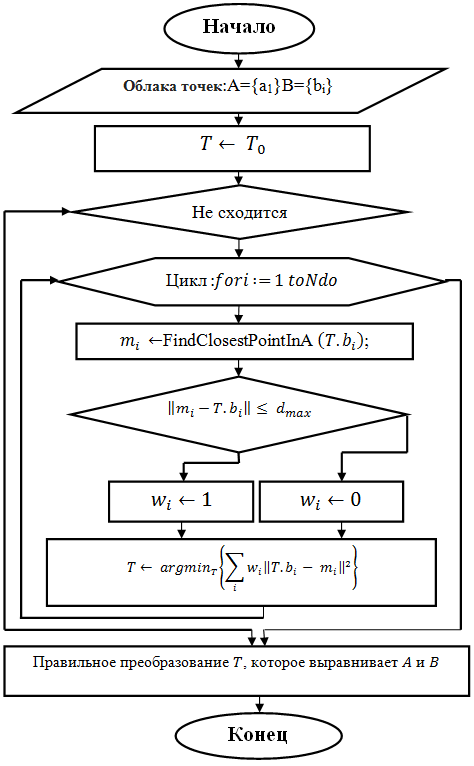
\includegraphics [scale=1] {images/h13.png}
\begin{center}
%\captionsetup{justification=justified, labelsep=period}
\caption{Блок-схема алгоритма $ICP$} \label{img13}
\end{center}
\end{figure}
В набор точек признаков, найденных на объекте, $29$ точек имеют признаки, извлеченные с атрибутами характерной геометрии: выпуклые, вогнутые кривые, соответствующие важным позициям, связанными с измерением размеров частей тела. Алгоритм включает в себя основные шаги:

\begin{itemize}
	\item \textbf{Шаг 1:} Вычислим соответствия между двумя сканированиями;
	\item \textbf{Шаг 2:} Выполним преобразование, которое сводит к минимуму расстояние между соответствующими точками.
\end{itemize}
Используем соответствующее максимальное пороговое значение $d_{max}$. Здесь $d_{max}$ представляет собой баланс между сходимостью и точностью.

Алгоритм $ICP$ повторяет действия, чтобы минимизировать среднеквадратичную ошибку пикселов, соответствующих ближайшей точке.
\begin{equation}\label{eq26}
T\leftarrow argmin_t\left\{\sum_i\left\|T.b_i - m_i\right\|^2\right\}.
\end{equation}
Где:

\begin{itemize}
	\item $T$ - правильное преобразование;
	\item $b_i$: $B=\left\{b_i\right\}$ - Облака точек;
	\item $m_i$ - множество точек, которые будут преобразованы из $B$ - $A$ ( $A=\left\{a_i\right\}$ - Облака точек);
\end{itemize}

Набор новых точек будет найден, если он удовлетворяет двум условиям:

\begin{itemize}
	\item Расположен на границе или наиболее близко к границам объекта;
	\item Расстояние между двумя наборами точек является наименьшим.
\end{itemize}
Таким образом, получен набор новых признаков для описания точного контура объекта.

Этапы алгоритма ICP выполнются последовательно. Алгоритм остановится только, если имеет место сходимость (наименьшая ошибка и стабильность). Алгоритм $ICP$ с такими операциями всегда монотонно сходится на интервале области определения функции. Тем не менее параметры алгоритма зависят от настройки. Таким образом, алгоритм $ICP$ будет сходиться на всей области определения функции. В то же время, новые точки признаков абсолютно совпадают с точками признаков в базе данных.